% id: 139-12
% book: 베이직쎈 미적분1 · 09 정적분의 활용
% section: 개념 56 곡선과 $x$축 사이의 넓이
% passage: 다음 주어진 구간에서 곡선과 두 직선 및 $x$축으로 둘러싸인 도형의 넓이를 구하시오.
% figure: tikz:fig-139-12
% answer: 
% answer_source: 
% variant_level: 0 (원본 전사)
% 이 파일은 build.mjs 가 items.json 에서 만든다. 고칠 때는 items.json 을 고친다.
\smash{\raisebox{1.5mm}{\dmkichul{베이직쎈 미적분1 139쪽 12번}}}
\noindent\begin{minipage}[t]{0.58\linewidth}\vspace{0pt}\raggedright $y=x^2-1$, $x=0$, $x=2$ \qquad $[0{,}\mkern3mu\mathopen{}2]$\end{minipage}\hfill\begin{minipage}[t]{0.4\linewidth}\vspace{0pt}\centering \resizebox{\ifdim\width>\linewidth\linewidth\else\width\fi}{!}{% 139-12(139쪽) — 포물선 $y=x^2-1$ 과 $x$축·두 직선 $x=0$, $x=2$ 로 둘러싸인 색칠 부분(0~1 은 축 아래, 1~2 는 축 위). 스캔 화질이 낮아 TikZ 로 다시 그림.
% 원문에 있는 것만 옮긴다: 곡선 · 색칠 부분 둘 · $x=2$ 세로선 · 라벨 $-1$, O, 1, 2($x$축), $-1$($y$값), $y=x^2-1$, x, y. 원문에 없는 눈금·넓이 값은 적지 않는다.
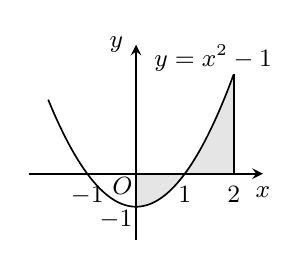
\begin{tikzpicture}[x=0.62cm, y=0.42cm, line width=0.6pt, font=\small]
  \fill[gray!20] (0,0) -- plot[domain=0:1, samples=40] (\x, {(\x)*(\x)-1}) -- (1,0) -- cycle;
  \fill[gray!20] (1,0) -- plot[domain=1:2, samples=40] (\x, {(\x)*(\x)-1}) -- (2,0) -- cycle;
  \draw[->, >=stealth, line width=0.7pt] (-2.2,0) -- (2.6,0) node[below=1pt] {$x$};
  \draw[->, >=stealth, line width=0.7pt] (0,-2.0) -- (0,3.9) node[left=1pt] {$y$};
  \draw[domain=-1.8:2.0, samples=90, smooth] plot (\x, {(\x)*(\x)-1});
  \draw (2,0) -- (2,3);
  \node[below=1pt] at (-1,0) {$-1$};
  \node[anchor=north east, inner sep=1pt] at (0,0) {$\pt{O}$};
  \node[below=1pt] at (1,0) {$1$};
  \node[below=1pt] at (2,0) {$2$};
  \node[anchor=north east, inner sep=1pt] at (0,-1) {$-1$};
  \node[anchor=west, inner sep=1pt] at (0.3,3.5) {$y=x^2-1$};
\end{tikzpicture}
}\end{minipage}\par
\dmhint{곡선 $y=x^2-1$과 $x$축의 교점의 $x$좌표는\\ $x^2-1=\blank$에서 \qquad $x^2=\blank$\\ $\therefore x=\blank$ 또는 $x=1$\\ 따라서 구하는 넓이는\\ $\displaystyle\int_{0}^{\text{\scriptsize\setlength{\fboxsep}{1.5pt}\framebox[1.5em]{\rule{0pt}{1.6ex}}}}|x^2-1|\mkern3mu dx$\\ $\displaystyle =\int_{0}^{\text{\scriptsize\setlength{\fboxsep}{1.5pt}\framebox[1.5em]{\rule{0pt}{1.6ex}}}}(-x^2+\blank)\mkern3mu dx+\int_{\text{\scriptsize\setlength{\fboxsep}{1.5pt}\framebox[1.5em]{\rule{0pt}{1.6ex}}}}^{2}(x^2-1)\mkern3mu dx$\\ $=\Big[-\dfrac{1}{3}x^3+\blank\Big]_{0}^{\text{\scriptsize\setlength{\fboxsep}{1.5pt}\framebox[1.5em]{\rule{0pt}{1.6ex}}}}+\Big[\dfrac{1}{3}x^3-x\Big]_{\text{\scriptsize\setlength{\fboxsep}{1.5pt}\framebox[1.5em]{\rule{0pt}{1.6ex}}}}^{2}$\\ $=\blank$}
